% H375 project technical report -- generated from archived experiment records.
\documentclass[UTF8,a4paper,11pt]{ctexrep}
\usepackage[a4paper,margin=2.2cm,headheight=15pt]{geometry}
\usepackage{amsmath,amssymb,bm,booktabs,longtable,tabularx,array,graphicx,float,xcolor}
\usepackage{tikz}
\usetikzlibrary{arrows.meta,positioning}
\usepackage{hyperref}
\usepackage{fancyhdr}
\usepackage{caption}
\hypersetup{colorlinks=true,linkcolor=blue!55!black,urlcolor=blue!55!black,
  pdftitle={epsilon-active 项目实验过程与 H375 求解流程技术报告}}
\graphicspath{{h375/figures/}}
\setlength{\parindent}{2em}
\setlength{\parskip}{0.28em}
\setlength{\emergencystretch}{3em}
\renewcommand{\arraystretch}{1.16}
\pagestyle{fancy}\fancyhf{}
\fancyhead[L]{epsilon-active 实验过程与 H375}
\fancyhead[R]{技术报告}
\fancyfoot[C]{\thepage}
\newcommand{\HPWL}{\operatorname{HPWL}}
\newcommand{\Overflow}{\operatorname{Overflow}}
\newcommand{\Excess}{\operatorname{excess}}
\newcommand{\Mcal}{\mathcal{M}}
\newcommand{\Bcal}{\mathcal{B}}
\newcommand{\Rcal}{\mathcal{R}}

\title{epsilon-active 项目实验过程与 H375 求解流程\\
\large 从密度可行化到精确 HPWL 恢复的分阶段研究}
\author{Huawei EDA Challenge 5 -- Global Placement}
\date{2026 年 8 月 30 日}

\begin{document}
\maketitle
\begin{abstract}
本报告总结 epsilon-active 全局布局项目的实验方法，并以 adaptec1 的 H375 为主线说明其完整求解流程。项目把困难分解为两个阶段：第一阶段从高度拥挤的连续初始布局中构造密度可接受的 checkpoint；第二阶段在严格 overflow 上界下恢复和优化精确 HPWL。该分解来自精确矩形/bin 交叠模型的一个基本事实：当单元位于 bin 内部、或多个过载 bin 之间需要协同迁移时，局部 density 次梯度会大面积为零，单纯提高密度系数不能产生长程搬运。

H375 的最终结果为 85.999318M HPWL、6.999990\% exact overflow。它不是单一参数设置，而是 ``静电同伦初始化 + exact 容量恢复 + 同形交换 polish'' 的 checkpoint 链。报告同时区分了方向选择与目标评价：epsilon-active 只用于选择精确 HPWL 的搜索方向；全部报告 HPWL 都是 pin-offset max--min 值，overflow 都来自精确矩形/bin 交叠。H375 尾端的同形交换并不调用 epsilon-active 梯度，而是直接以精确 HPWL 增量接受交换。
\end{abstract}
\tableofcontents

\chapter{问题、模型与两阶段总述}
\section{为何采用两阶段}
设可移动单元集合为 $\Mcal$，布局区域为 $\Rcal$，网集合为 $\mathcal{E}$。pin $p$ 的坐标包含 Bookshelf offset：
\[
 X_p=x_{n(p)}+\Delta x_p,\qquad Y_p=y_{n(p)}+\Delta y_p.
\]
前向线长始终是精确 HPWL：
\begin{equation}
 W(\bm{x})=\sum_{e\in\mathcal E}w_e\left(\max_{p\in e}X_p-\min_{p\in e}X_p+
 \max_{p\in e}Y_p-\min_{p\in e}Y_p\right).\label{eq:hpwl}
\end{equation}
对 bin $b\in\Bcal$，占用是 movable rectangles 与 physical fixed macros 的精确相交面积 $u_b$。令 $A_b$ 为 bin 面积、目标密度为 $\rho_t=1$，则
\begin{equation}
 D(\bm{x})=\frac12\sum_{b\in\Bcal}\frac{[u_b-\rho_tA_b]_+^2}{A_b},\qquad
 \Overflow(\bm{x})=\frac{\sum_{b\in\Bcal}[u_b-\rho_tA_b]_+}{\sum_{i\in\Mcal}w_ih_i}.\label{eq:density}
\end{equation}
固定 macro 进入 $u_b$，而 \texttt{terminal\_NI} 不占物理容量。密度项的局部导数含有 $\partial |R_i\cap b|/\partial x_i$。若矩形完整落在 bin 内部，此导数可为零；若源/目的均过载，移动可能降低平方 excess 而不降低总 overflow。这就是密度优化的 ``active-set starvation''，也是两阶段分解的动机。

第一阶段的目标是跨越零梯度平台并到达低 overflow basin；第二阶段则将布局限制在 $\Overflow\leq 0.07$ 的可行带中，尽量修复第一阶段造成的拓扑损失。两阶段不是把目标替换为平滑 surrogate：所有 checkpoint 都由式~\eqref{eq:hpwl}--\eqref{eq:density} 审计。

\section{H375 总体链条}
\begin{center}
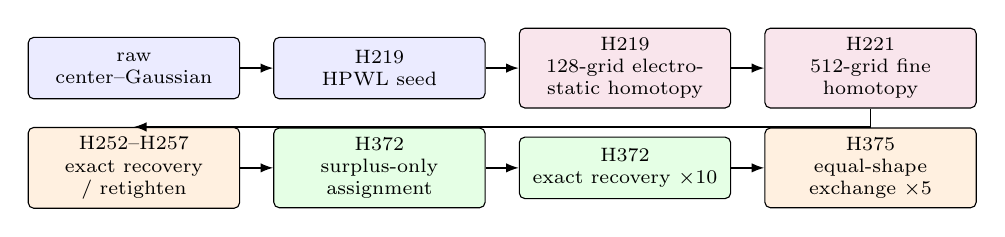
\begin{tikzpicture}[node distance=0.35cm and 0.42cm, every node/.style={draw,rounded corners=2pt,align=center,font=\scriptsize,minimum height=0.78cm,text width=2.45cm}, arr/.style={-{Latex[length=1.6mm]},line width=.55pt}]
\node[fill=blue!8] (r) {raw\\center--Gaussian};
\node[fill=blue!8,right=of r] (s) {H219\\HPWL seed};
\node[fill=purple!10,right=of s] (c) {H219\\128-grid electrostatic homotopy};
\node[fill=purple!10,right=of c] (f) {H221\\512-grid fine homotopy};
\node[fill=orange!12,below=of r] (a) {H252--H257\\exact recovery / retighten};
\node[fill=green!10,right=of a] (b) {H372\\surplus-only assignment};
\node[fill=green!10,right=of b] (q) {H372\\exact recovery $\times10$};
\node[fill=orange!12,right=of q] (x) {H375\\equal-shape exchange $\times5$};
\draw[arr] (r)--(s); \draw[arr] (s)--(c); \draw[arr] (c)--(f);
\draw[arr] (f.south)|-(a.north); \draw[arr](a)--(b); \draw[arr](b)--(q); \draw[arr](q)--(x);
\end{tikzpicture}
\end{center}
其中 H219/H221 是达到可接受密度的长程初始化；H252 之后逐步进入精确非光滑尾部。完整归档时间为 236.40 s；H375 的最后五轮交换耗时 37.63 s。

\chapter{第一阶段：密度可行化与零梯度问题}
\section{epsilon-active 的角色}
对每条网，epsilon-active 并不改变式~\eqref{eq:hpwl}，而是在靠近极值的 pin 间分配搜索方向。例如最大端的权重为
\begin{equation}
 a^{\max}_{p,x}=\left[1-\frac{x_e^{\max}-X_p}{\epsilon}\right]_+^q,
 \qquad
 g_{p,x}=w_e\left(\frac{a^{\max}_{p,x}}{\sum_ra^{\max}_{r,x}}-
 \frac{a^{\min}_{p,x}}{\sum_ra^{\min}_{r,x}}\right).\label{eq:epsactive}
\end{equation}
它缓和 net 极值身份频繁切换，却不能独自解决密度交叠的零梯度。因此研究的重点不是无限扩大 $\epsilon$，而是构造能够越过几何断点、或产生长程连续力的密度方向。

\section{主路径：静电同伦 H219--H221}
静电同伦把精确目标保留为审计基准，并在早期附加一个会产生长程力的辅助项：
\begin{equation}
 F_{\mu}=\frac{W}{W_0}+\lambda\frac{D}{D_0}+
 \mu\left(\frac{E_{\rm el}}{E_0}+\kappa\frac{\|\bm{x}-\bm{x}_c\|_2^2}{A_0}\right),
 \qquad -\nabla^2\phi=\rho,\quad \bm E=-\nabla\phi.\label{eq:homotopy}
\end{equation}
这里 $E_{\rm el}$ 由 DCT/Poisson 求解，中心锚点消除 Neumann 平移零模。$\mu$ 随 stage 衰减到零，$\lambda$ 在接近可行带时承担精确 overlap 约束。动机是：电场对远处的过载也给出连续方向，能使单元离开 ``整块落在同一 bin'' 的平坦区域；最终 $\mu=0$，因此报告的最终值不依赖电势能。

H219 先以 HPWL-only Adam 得到 43.035M/96.056\%，再在 128$\times$128 grid 经 24$\times$50 step 同伦到 60.617M/71.708\%。H221 将该 checkpoint 升至 512$\times$512，采用更强的物理尺度校准，得到 109.426M/7.752\% 的低 overflow 入口。图~\ref{fig:homotopy} 展示归档的 coarse/fine 收敛曲线。该路径是 H375 能进入 7\% 邻域的关键，但应如实说明：它是静电辅助初始化，不是全程纯 exact-overlap 求解。
\begin{figure}[H]\centering
\includegraphics[width=.94\textwidth]{fig_homotopy_detail.png}
\caption{H219/H221 静电同伦的归档轨迹：$\mu$ 早期提供长程扩散，末阶段退至零，exact HPWL 与 exact overflow 始终单独记录。}\label{fig:homotopy}
\end{figure}

\section{其他 density-only / density-first 方案及其动机}
\begin{longtable}{p{2.3cm}p{4.8cm}p{4.4cm}}
\toprule 方案 & 如何对抗零梯度 & 结果与结论\\\midrule\endhead
H52--H54：density epsilon continuation & 先让 8-bin 邻域的 overlap active pieces 提供方向，再逐次缩至 4、2 bin。动机是减少远处片段相互抵消，同时保留跨 bin 边界的可见性。 & overflow 从 96.89\% 降至 38.82\%，但 HPWL 升至 1204.24M；固定 epsilon 下仍振荡，说明非局部伪方向不是 exact density 的稳定下降方向。\\
H58：exact breakpoint coordinate & 枚举单元跨越矩形/bin 折点的位置，直接跳过 ``bin 内部导数为零'' 的平坦段；仅接受 exact overflow 和 energy 同降的候选。 & 20 sweep 仅到 94.73\%。机制几何上正确，但严格 overflow 单调性拒绝了过载 bin 间的中性转运。\\
H67：vector bin prices & 对每个 bin 建立价格场，候选 block 沿 ``从高价过载区到低价区'' 的方向移动。动机是用空间非均匀 dual signal 取代单一 $\lambda$，激活协同块。 & 单调降至 83.13\%，但 HPWL 到 204.57M；价格没有编码二维 net 连通性。\\
H68：64-to-512 multilevel breakpoint & 先在粗网格上移动，粗 bin 可以跨越细网格大量断点；再在细网格精确审计。动机是改变几何尺度而非平滑目标。 & 达 69.27\%，优于 H67，但 coarse assignment 已破坏拓扑，HPWL 341.72M。\\
H100：宽半径 exact breakpoint + recovery & 将可见 breakpoint 半径扩到 64 bin，并在每轮 density refinement 后以 overflow cap 恢复 HPWL。动机是把局部零梯度问题转化为有限的、可审计的远程候选搜索。 & 第三轮达到 6.24086\%；首次得到严格可行 checkpoint，但运行时间和 HPWL 均不适合作为 H375 主前缀。\\
\bottomrule
\end{longtable}
这些实验的共同结论是：问题不只是 ``density 权重不够大''。有效方案必须同时处理两件事：跨过 active-set 断点，以及保护 net topology。静电同伦负责前者的连续长程驱动，H372 的容量分配和后续恢复负责后者。

\chapter{第二阶段：HPWL 联合优化与 H375 尾部}
\section{从 H221 到 H257：先松后紧地进入 7\% 带}
H252 从 H221 的 7.8\% checkpoint 出发，先把 overflow cap 放宽到 15\%。动机是给 coordinated moves 留出 ``density slack''，避免一开始就在 7\% 边界上因无可行动作而停滞。两轮 exact breakpoint/compact/net-block recovery 到 94.549M/15.000\%。

H253 使用中等 density weight（0.5）和 net-share direction 做 81 次 bridge，动机是让同网单元共享局部密度方向，避免每个 cell 独立撤离导致割裂。随后 H254 将 density scale 提至 4.75 执行强 retighten，得到 89.549M/6.557\%。H255/H257 再关掉 density 连续优化，改用 axis-separated breakpoint 与 compact candidate；每一候选均需满足 $\Overflow\leq0.07$ 且精确 HPWL 下降。其最终达到 87.119M/6.99996\%。

\section{H372：容量修复后在可行带内恢复 HPWL}
H372 从 H257 出发执行 position-seeded surplus-only recursive bisection。它只移动为满足固定 macro 感知容量上界所必需的 boundary surplus，而不是重新全局排序；叶子采用 nearest-capacity 和 HPWL-guided assignment。动机是将密度修复限制为必要最小集合，保护已有 net 相对几何。该步骤暂时把 HPWL 提至 93.705M，但 overflow 降为 2.306\%，创造了可消费的 slack。

之后 H372 进行十轮 exact recovery：epsilon-active HPWL 方向（$\epsilon=85,q=4$）用于产生候选；axis-separated breakpoint、compact direction 与 net-block density direction 提供跨零梯度的有限候选；每次提交前都以精确 HPWL delta 和 exact overflow cap 审核。十轮得到 86.190M/6.99999\%。图~\ref{fig:tail} 显示 exact tail 的单调恢复过程。
\begin{figure}[H]\centering
\includegraphics[width=.92\textwidth]{fig_exact_tail.png}
\caption{H372 容量 assignment、十轮 exact recovery 与 H375 最终交换。}\label{fig:tail}
\end{figure}

\section{H375：同形、net-aware 精确交换}
H375 最终从 H372 recovery10 的 \texttt{last.pl} 开始，执行五轮交换。仅允许宽高相同的 movable cells 交换位置，因而每个 bin 的矩形多重集不变，理论上 density occupancy 与 overflow 不变。对候选 $a,b$，接受条件是
\begin{equation}
 \Delta W_{a\leftrightarrow b}=W(\bm{x}^{a\leftrightarrow b})-W(\bm{x})<0,
 \qquad \Delta\Overflow=0.\label{eq:swap}
\end{equation}
实现优先从 node 的 incident nets 中找同形对象，再补充以目标位置为中心、半径 64 bin 的空间候选；每个 node 至多 32 个候选，精确 shortlist 为 16，net degree limit 为 1000。动机是把最后的优化限制为不破坏容量的 topology polish，而不是再进行密度搬运。

五轮分别接受 8064、3415、1651、812、429 次交换，HPWL 从 86.189626M 降到 \textbf{85.999318M}，overflow 保持 6.999990\%。注意本阶段不使用 epsilon-active 梯度；它是 exact HPWL delta 搜索。完整曲线见图~\ref{fig:full}。
\begin{figure}[H]\centering
\includegraphics[width=.94\textwidth]{fig_full_chain_convergence.png}
\caption{H375 全链条 checkpoint 轨迹。不同颜色对应初始化、同伦、exact recovery 与交换阶段，不能误读为单次 Adam 迭代。}\label{fig:full}
\end{figure}

\section{联合优化的其他有代表性的方案}
\begin{longtable}{p{2.5cm}p{5.0cm}p{4.0cm}}
\toprule 方案 & 动机 & 结论\\\midrule\endhead
H76--H78 adaptive homotopy & 将 $\mu$ 衰减与 $\lambda$ 增长绑定到 overflow window，避免固定退火过快失去长程力、过慢又长期偏离 exact 目标。 & H78 达 56.33\%，证明状态触发优于固定日程，但仍需要 topology-aware capacity stage。\\
H94/H96 wide-breakpoint cycles & 扩大 breakpoint 可见半径，以更大 HPWL 代价换取穿越低梯度岛的能力；每个 cycle 后在固定 overflow cap 下做 HPWL recovery。 & 可大幅推进可行性，但 HPWL/runtime 代价高，适合作为机制证据。\\
H102 equal-shape swaps & 在已有可行点上保持 rectangle anchor multiset 不变，只优化 incident-net 的精确 HPWL。 & 证实 ``先可行、后无密度变化 polish'' 有效，是 H375 的直接前身。\\
H376 relaxed-to-15\% then retighten & 测试更大 slack 是否能跳到更好的 HPWL basin。 & 可短暂到 83.820M，但直接收紧停在 14.87\%；可行 basin 与 relaxed basin 不连通。\\
H403 ablation & 从同一 H372 checkpoint 分离 node move、breakpoint、compact、net-block 与 exchange 的贡献。 & net-block density direction 是最强孤立 recovery 成分；exchange 是小但昂贵的最终 polish。\\
\bottomrule
\end{longtable}

\chapter{固定参数 H375 重放：adaptec1--4}
为验证该链条不是只对 adaptec1 有效，本文在同一台主机上按顺序重放 adaptec1--4。四个数据集使用完全相同的 H375 参数与 stage handoff；计时为各求解器内部 \texttt{seconds} 的和，不含进程启动、目录创建与文本 I/O。表~\ref{tab:replay} 同时记录细同伦出口、H372 recovery10 与 H375 最终结果，因此可区分 ``进入可行带'' 和 ``尾部 HPWL 修复'' 的贡献。

\begin{table}[H]
\centering\small
\caption{2026-08-30 固定参数 H375 重放。HPWL 单位为 M；overflow 为精确 grid overlap 比例。}\label{tab:replay}
\begin{tabular}{lrrrrrrr}
\toprule
数据集 & \multicolumn{2}{c}{H221 fine} & \multicolumn{2}{c}{H372 rec$\times10$} & \multicolumn{2}{c}{H375 final} & 总计时 (s)\\
 & HPWL & overflow & HPWL & overflow & HPWL & overflow & \\\midrule
adaptec1 & 109.838 & 7.770\% & 89.309 & 7.000\% & \textbf{88.647} & 7.000\% & 179.706\\
adaptec2 & 140.280 & 4.126\% & 102.340 & 7.000\% & \textbf{101.781} & 7.000\% & 202.873\\
adaptec3 & 731.604 & 11.472\% & 369.210 & 7.000\% & \textbf{360.856} & 7.000\% & 337.639\\
adaptec4 & 657.376 & 6.934\% & 264.678 & 7.000\% & \textbf{263.352} & 7.000\% & 352.237\\
\bottomrule
\end{tabular}
\end{table}

四例均被尾部 recovery 拉回 7\% 可行带，且五轮交换进一步降低 HPWL（a1/a2/a3/a4 分别降低 0.662/0.558/8.354/1.327 M）。总阶段内时间为 180--352 s，随 netlist 规模与尾部精确候选数增长。这里的数值是\emph{固定参数迁移重放}，而非逐 benchmark 再调参后的最好成绩；尤其 adaptec1 的重放为 88.647M，与归档 H375 的 85.999M 不同，说明 H219/H221 的二进制版本、输入 checkpoint 与 snapshot 选择会显著影响最终 basin。因此该表提供可复现的端到端基线，不应替代归档最优记录。

\chapter{结论与复现建议}
H375 的成功不是某个单独超参数，而是按职责分工的链条：静电同伦解决早期长程密度扩散；15\% relaxed band 与 strong retighten 构造 7\% 可行入口；surplus-only assignment 用最少的容量移动重建 slack；epsilon-active recovery 在精确约束下恢复 HPWL；同形交换在不改变 density 的条件下做最终细化。

若要迁移到另一项目，建议将 ``精确 oracle + H372 recovery + H375 exchange'' 封装为独立 tail optimizer；不要仅复制交换代码并将其称为 H375 复现。完整 raw-to-H375 链还依赖归档的 H219/H221 电势同伦驱动和 checkpoint 选择策略。

\begin{thebibliography}{9}
\bibitem{h375} epsilon-active, \emph{H375 Complete Chain Technical Report}, archived experiment report, 2026.
\bibitem{h72} epsilon-active, \emph{H72--H73 Electrostatic Homotopy Results}, experiment analysis, 2026.
\bibitem{dreamplace} Y. Lin et al., ``DREAMPlace: Deep Learning Toolkit-Enabled GPU Acceleration for Modern VLSI Placement,'' \emph{IEEE TCAD}, 2021.
\bibitem{eplace} J. Lu et al., ``ePlace: Electrostatics-Based Placement Using Fast Fourier Transform and Nesterov's Method,'' \emph{TODAES}, 2015.
\end{thebibliography}
\end{document}
